%\documentclass[a4paper]{article}
\usepackage[utf8]{inputenc}
\usepackage[spanish, es-tabla, es-noshorthands]{babel}
\usepackage[table,xcdraw]{xcolor}
\usepackage[a4paper, footnotesep=1.25cm, headheight=1.25cm, top=2.54cm, left=2.54cm, bottom=2.54cm, right=2.54cm]{geometry}
%\geometry{showframe}

%\usepackage{wrapfig}			%Wrap figure in text
\usepackage[export]{adjustbox}	%Move images
\usepackage{changepage}			%Move tables

\usepackage{tikz}
\usepackage{amsmath}
\usepackage{amsfonts}
\usepackage{amssymb}
\usepackage{float}
\usepackage{graphicx}
\usepackage{caption}
\usepackage{subcaption}
\usepackage{multicol}
\usepackage{multirow}
\usepackage{wrapfig}
\setlength{\doublerulesep}{\arrayrulewidth}
\usepackage{booktabs}
\usepackage[numbib, nottoc, notlot, notlof]{tocbibind}

\usepackage{hyperref}
\hypersetup{
    colorlinks=true,
    linkcolor=blue,
    filecolor=magenta,      
    urlcolor=blue,
    citecolor=blue,    
}

%Change Font Size

% #1 = size, #2 = text
\newcommand{\setparagraphsize}[2]{{\fontsize{#1}{6}\selectfont#2 \par}}		%Cambia el size de todo el parrafo
\newcommand{\setlinesize}[2]{{\fontsize{#1}{6}\selectfont#2}}				%Cambia el font de una oración

\newcommand{\note}[1]{
	\begin{center}
		\huge{ \textcolor{red}{#1} }
	\end{center}
}

%FONTS (IMPORTANTE): Compilar en XeLaTex o LuaLaTeX
\usepackage{anyfontsize}	%Font size
\usepackage{fontspec}		%Font type

\usepackage{etoolbox}
\usepackage{todonotes}

\newcommand{\observacion}[2]{  \ifnumequal{1}{#1}{ { \todo[inline,backgroundcolor=red!25,bordercolor=red!100]{\textbf{Observación: #2}} } }{  }  }

\setcounter{topnumber}{2}
\setcounter{bottomnumber}{2}
\setcounter{totalnumber}{4}
\renewcommand{\topfraction}{0.85}
\renewcommand{\bottomfraction}{0.85}
\renewcommand{\textfraction}{0.15}
\renewcommand{\floatpagefraction}{0.8}
\renewcommand{\textfraction}{0.1}
\setlength{\floatsep}{5pt plus 2pt minus 2pt}
\setlength{\textfloatsep}{5pt plus 2pt minus 2pt}
\setlength{\intextsep}{5pt plus 2pt minus 2pt}

\newcommand{\quotes}[1]{``#1''}
\usepackage{array}
\newcolumntype{C}[1]{>{\centering\let\newline\\\arraybackslash\hspace{0pt}}m{#1}}
\usepackage[american]{circuitikz}
\usetikzlibrary{calc}
\usepackage{fancyhdr}
\usepackage{units} 

\graphicspath{{../Control de posición no lineal/}{../Control de fuerza no lineal/}{../Control híbrido no lineal/}{../Referencias/}{../Deducción de modelo/}{../Conclusiones/}}

\pagestyle{fancy}
\fancyhf{}
\lhead{22.99 - Automación Industrial}
\rhead{Lambertucci, Londero B., Maselli, Mechoulam}
\rfoot{Página \thepage}

%Items con bullets y no cuadrados
\renewcommand{\labelitemi}{\textbullet }

%
%\begin{document}
\Subsection{Realimentación de Estados}

\begin{figure}[H]
	\centering
	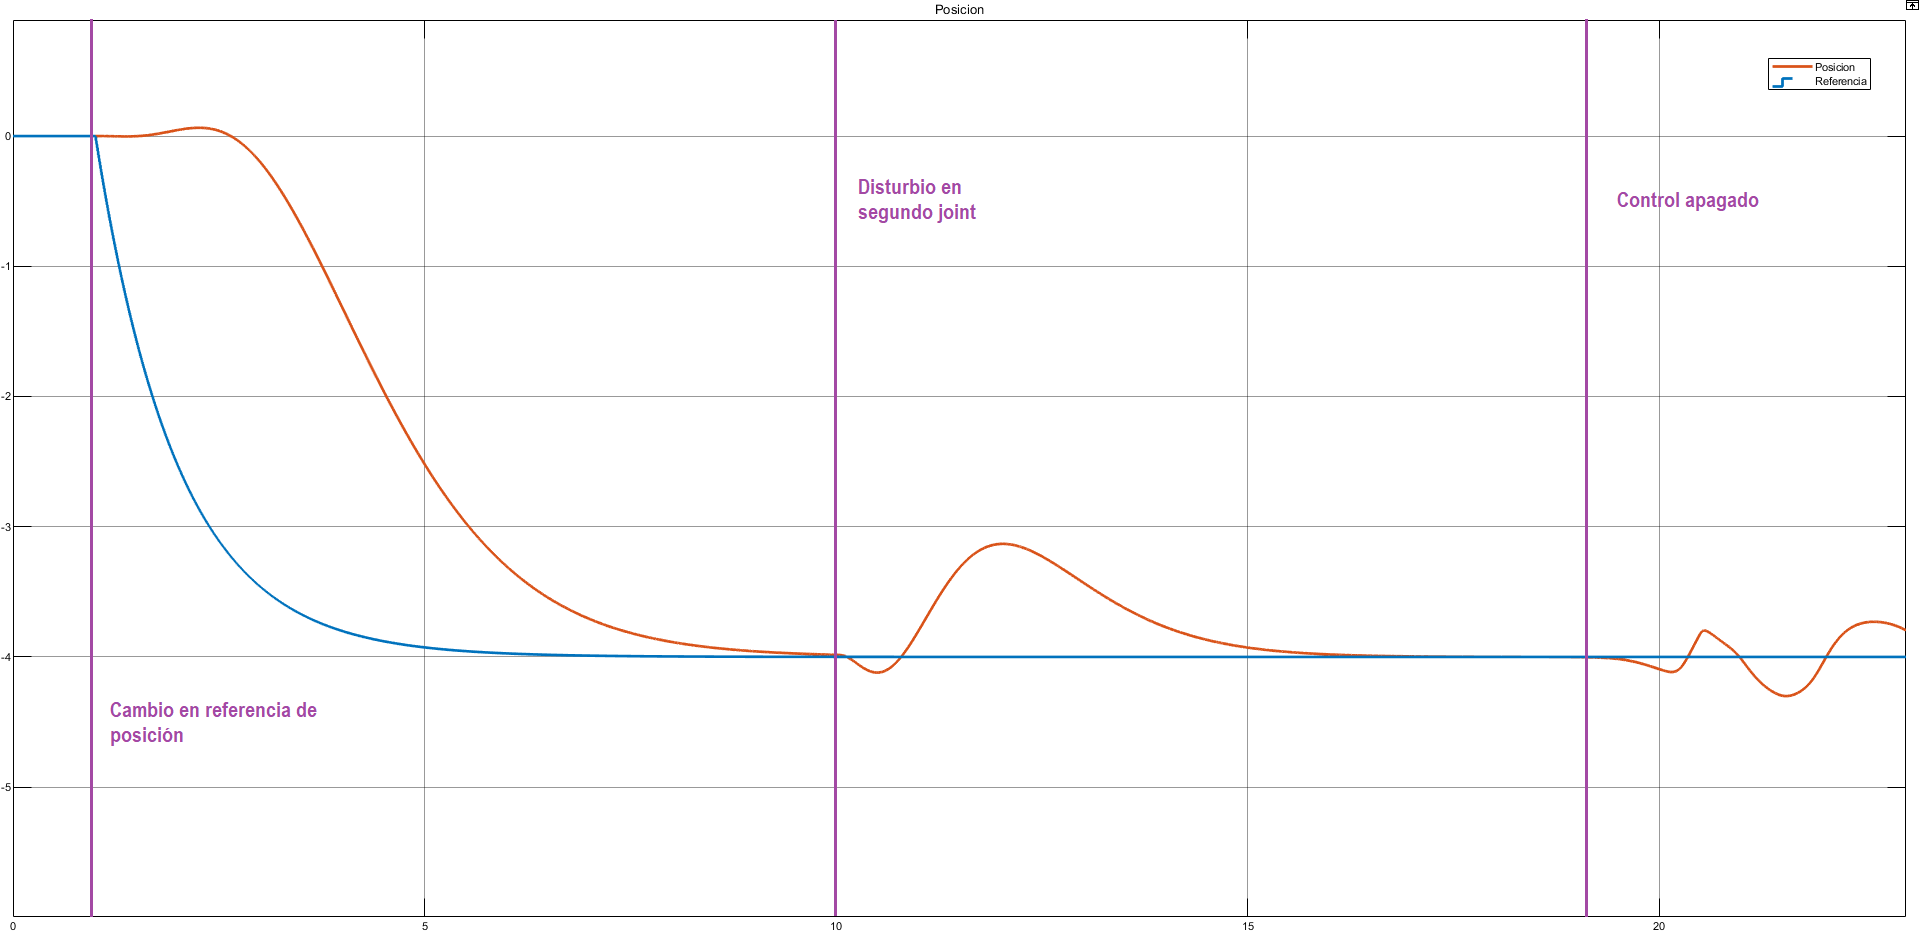
\includegraphics[width=\linewidth]{../Analisis de Resultados/ImagenesAnalisis de Resultados/realim_posref.png}
	\caption{pendiente.}	
	\label{fig:realim_posref}
\end{figure}

\begin{figure}[H]
	\centering
	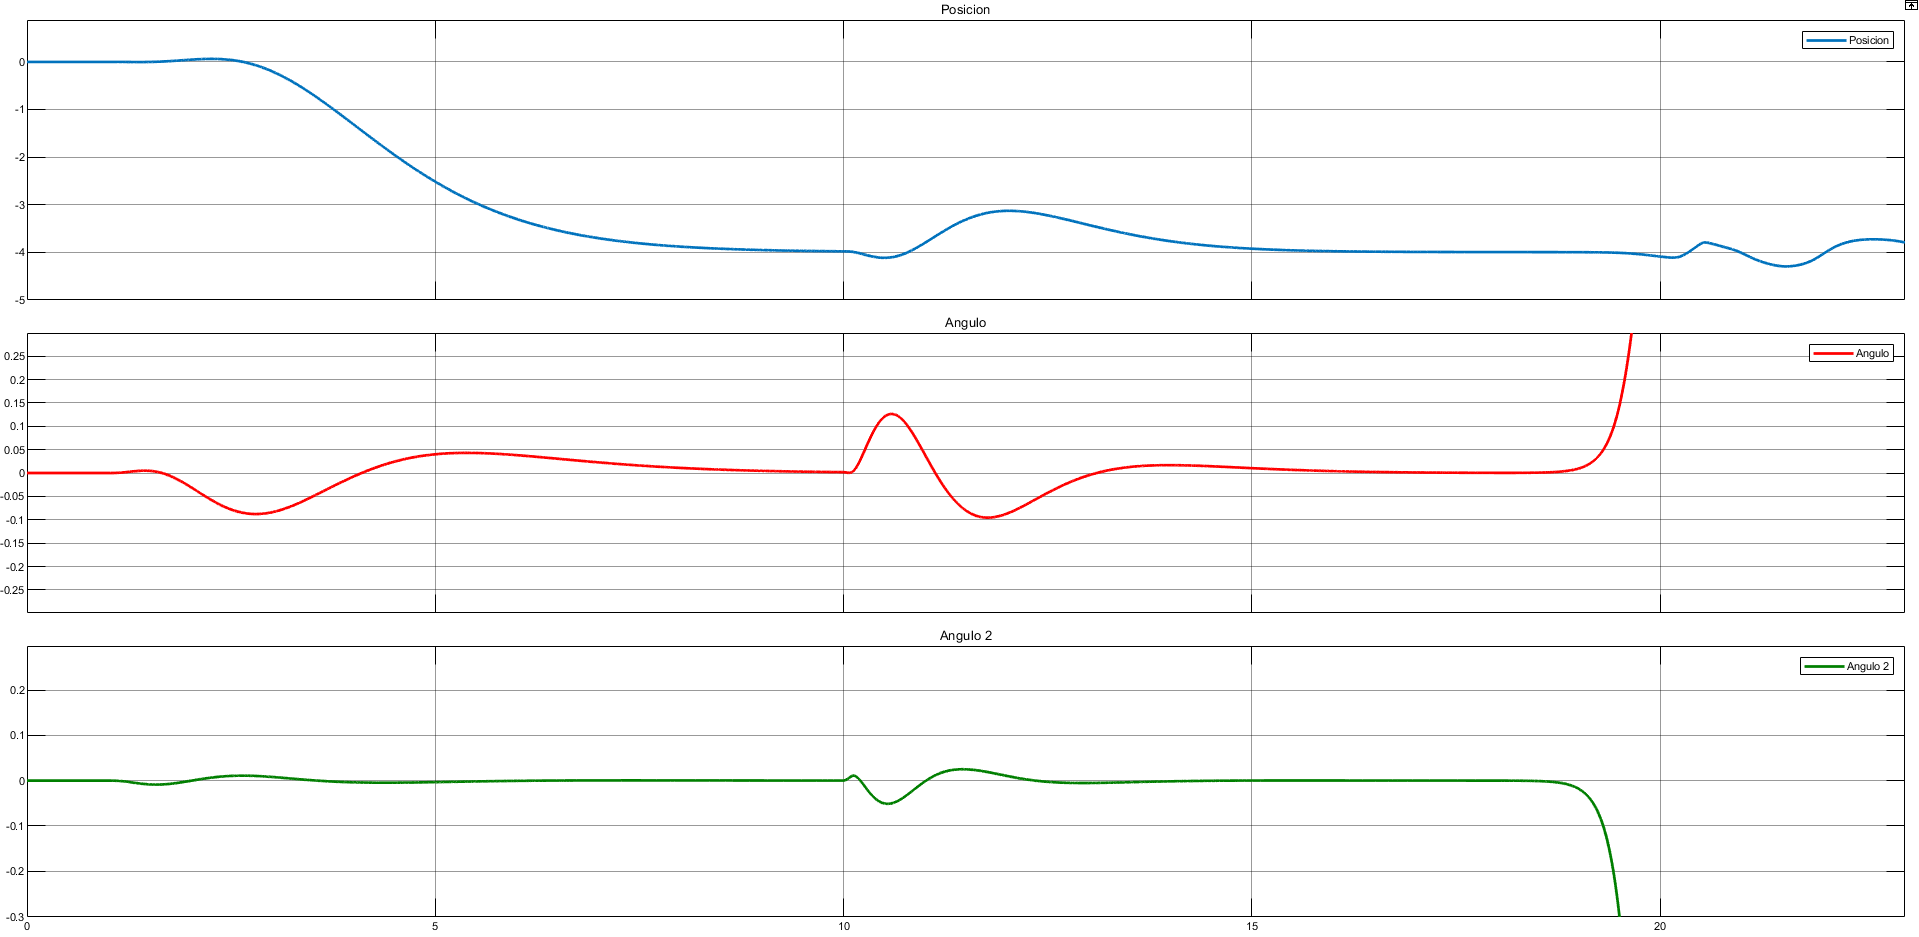
\includegraphics[width=\linewidth]{../Analisis de Resultados/ImagenesAnalisis de Resultados/realim_vars.png}
	\caption{pendiente.}	
	\label{fig:realim_vars}
\end{figure}

\Subsection{Observador}

\begin{figure}[H]
	\centering
	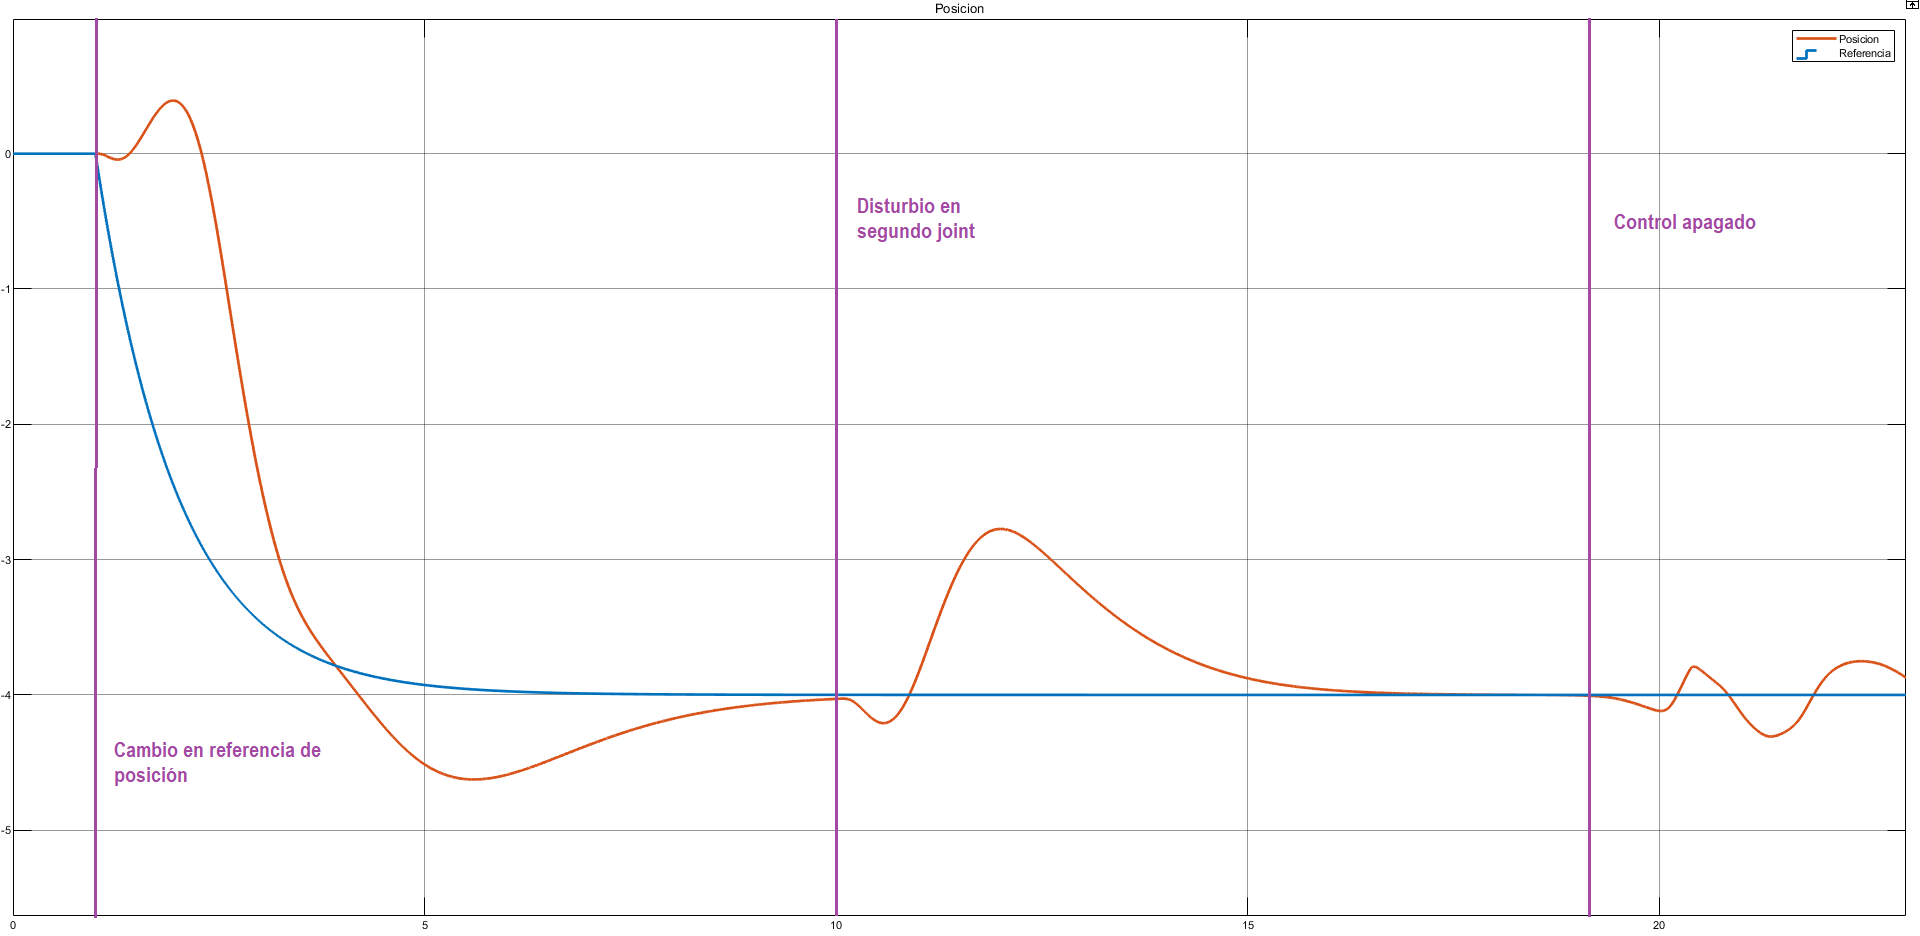
\includegraphics[width=\linewidth]{../Analisis de Resultados/ImagenesAnalisis de Resultados/obsv_posref.png}
	\caption{pendiente.}	
	\label{fig:obsv_posref}
\end{figure}

\begin{figure}[H]
	\centering
	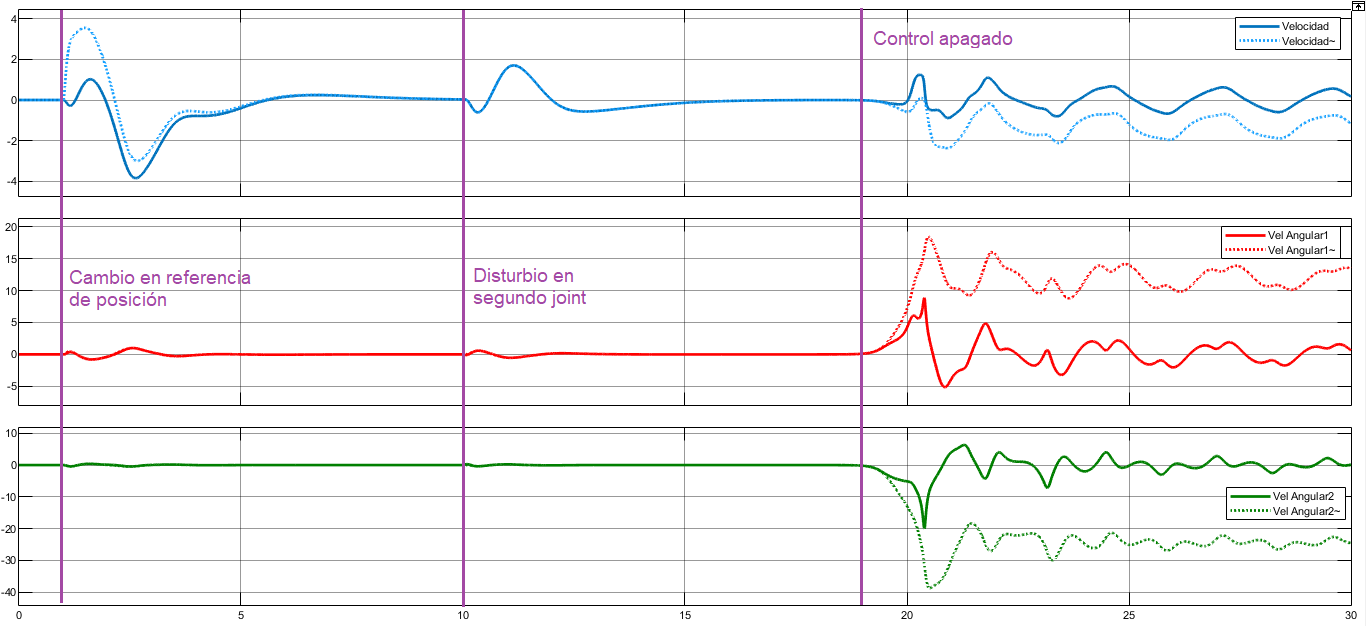
\includegraphics[width=\linewidth]{../Analisis de Resultados/ImagenesAnalisis de Resultados/obsv_vars.png}
	\caption{pendiente.}	
	\label{fig:obsv_vars}
\end{figure}

\Subsection{Discretización}

\begin{figure}[H]
	\centering
	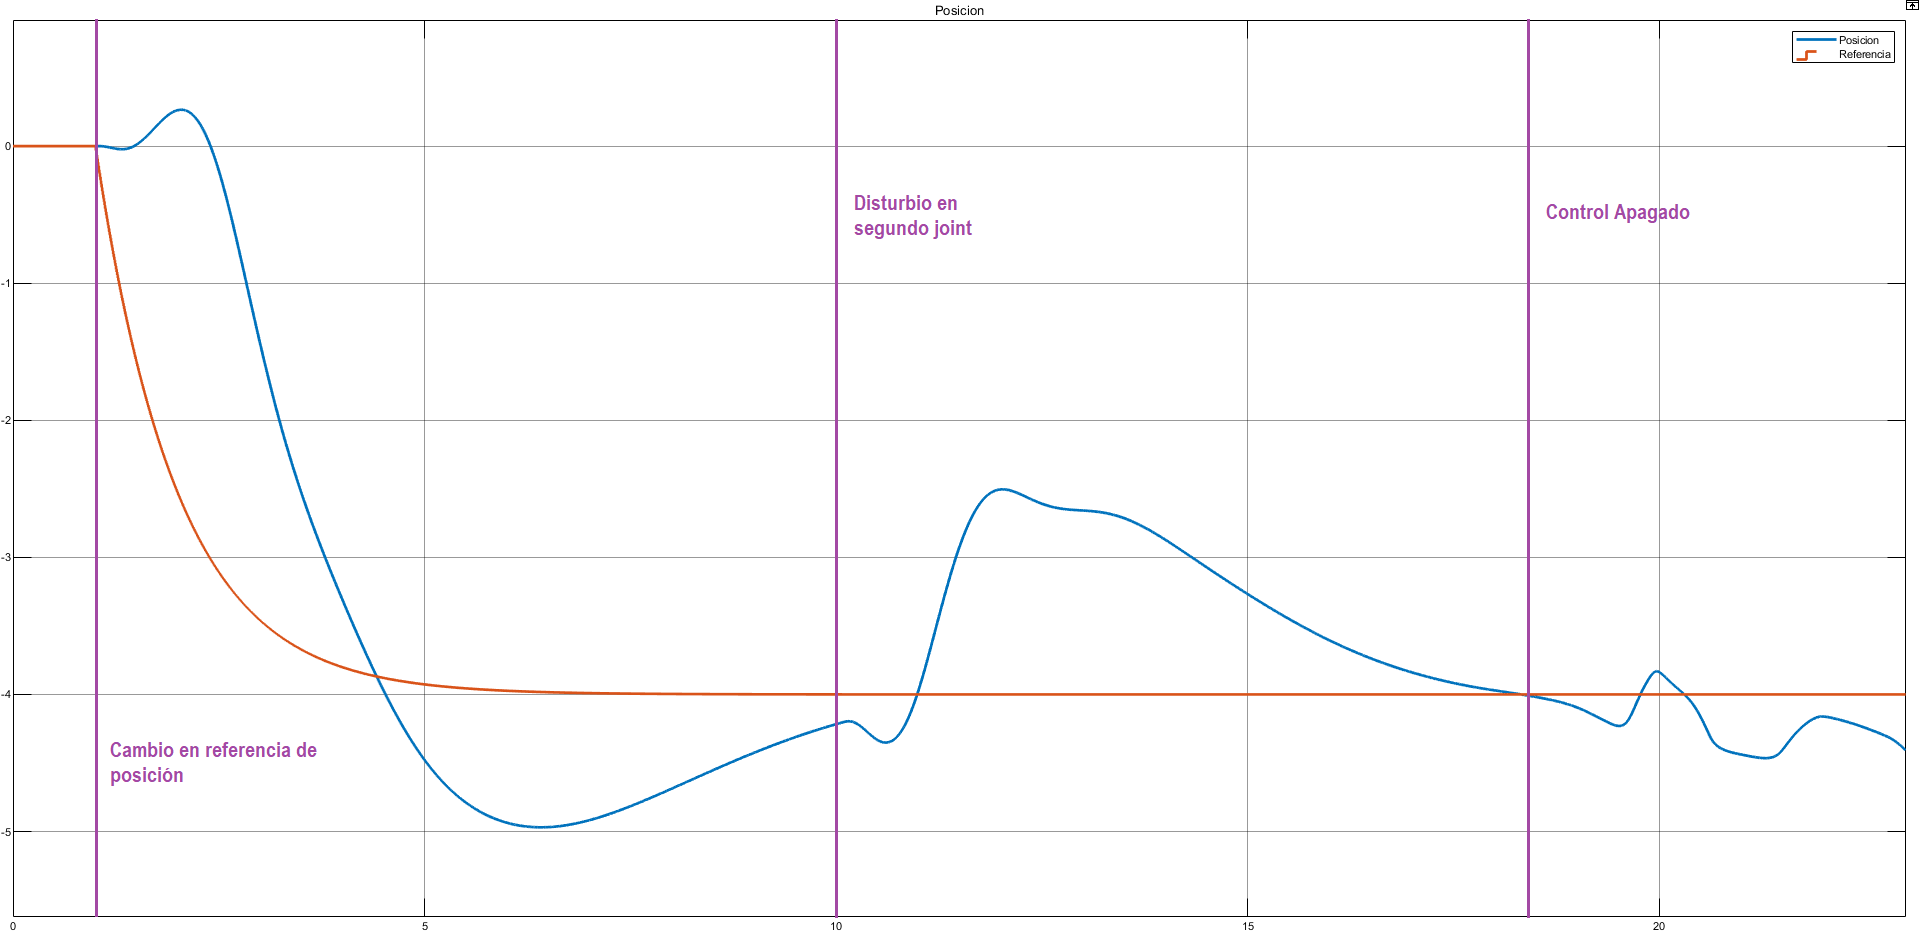
\includegraphics[width=\linewidth]{../Analisis de Resultados/ImagenesAnalisis de Resultados/obsv_disc_posref.png}
	\caption{pendiente.}	
	\label{fig:obsv_disc_posref}
\end{figure}

\begin{figure}[H]
	\centering
	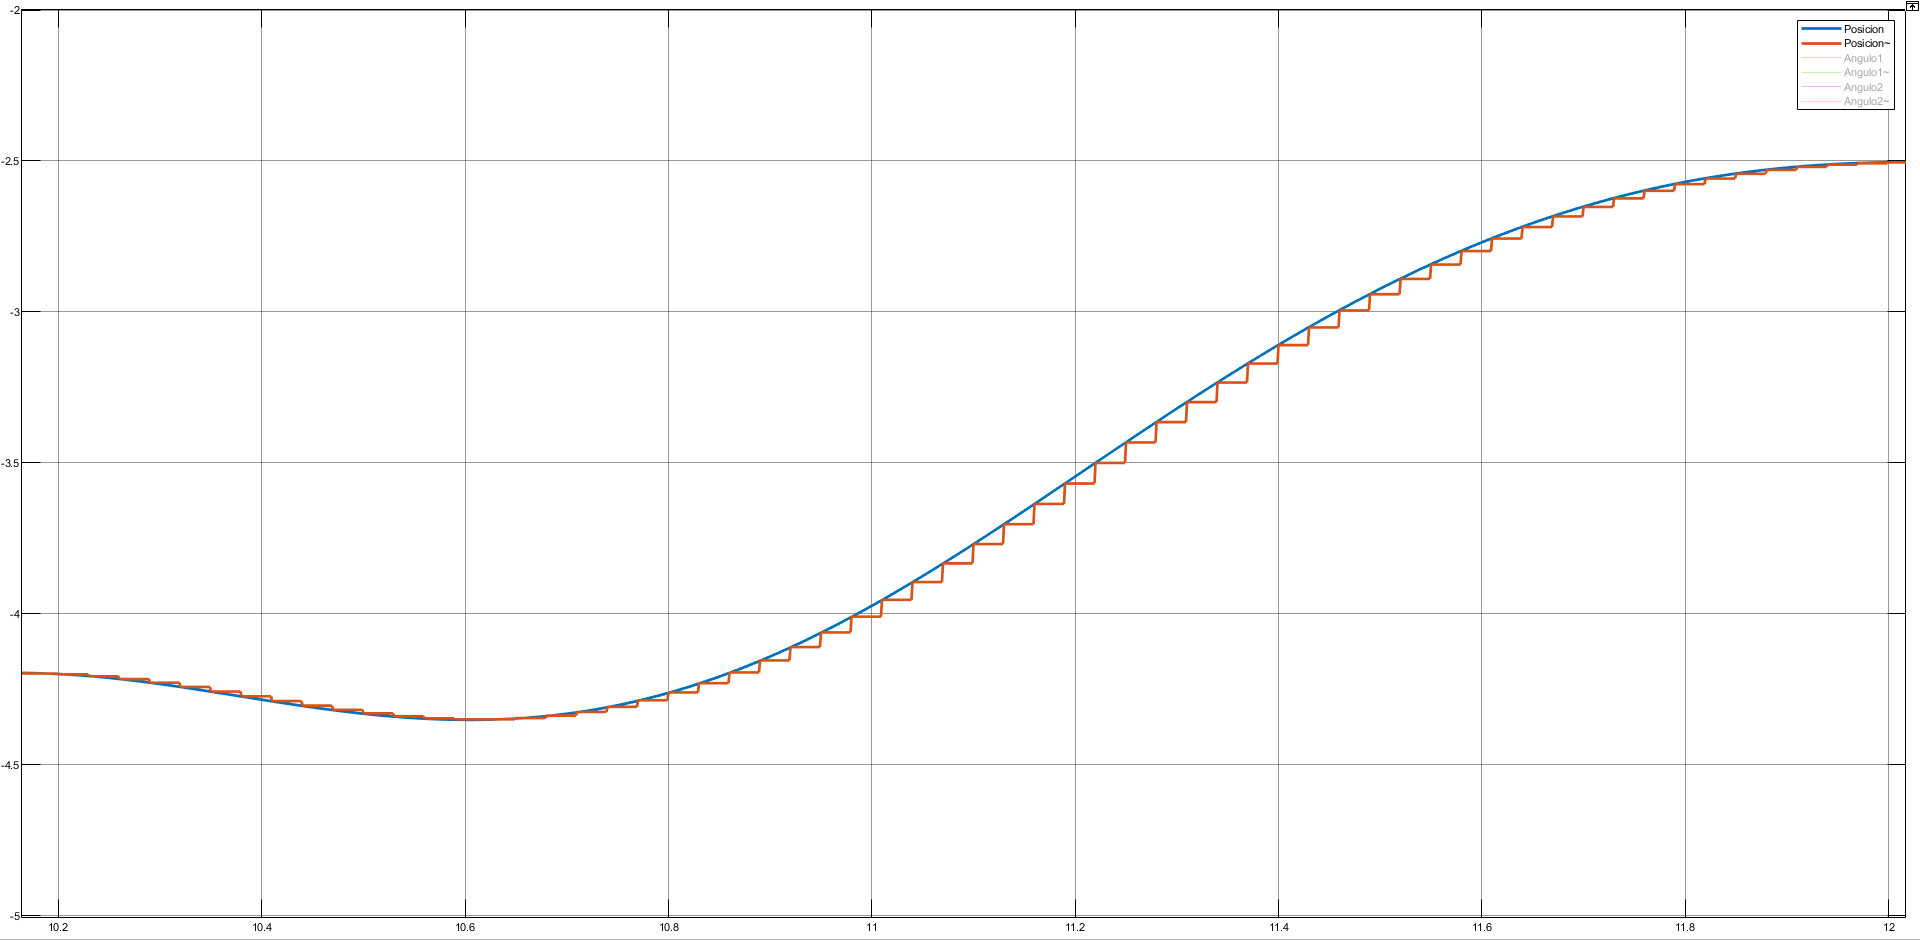
\includegraphics[width=\linewidth]{../Analisis de Resultados/ImagenesAnalisis de Resultados/obsv_disc_posdisc.png}
	\caption{pendiente.}	
	\label{fig:obsv_disc_posdisc}
\end{figure}

\begin{figure}[H]
	\centering
	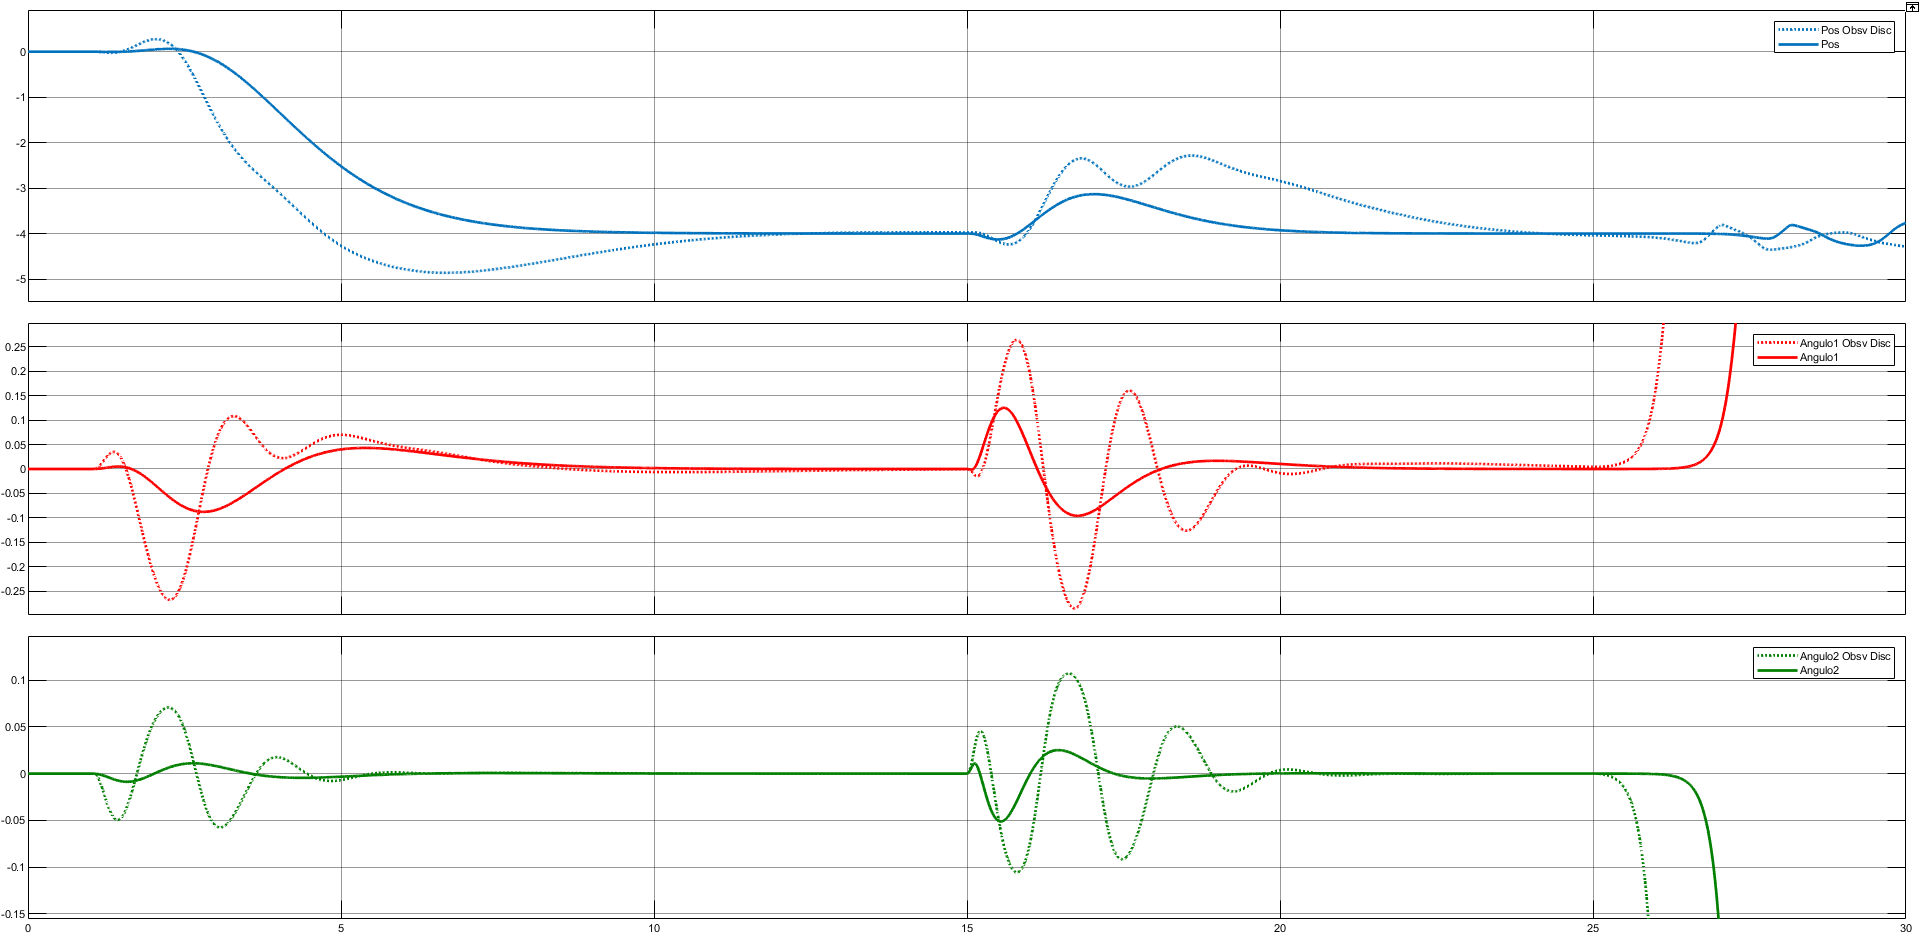
\includegraphics[width=\linewidth]{../Analisis de Resultados/ImagenesAnalisis de Resultados/disc_vs_ideal_vars.png}
	\caption{pendiente.}	
	\label{fig:disc_vs_ideal_vars}
\end{figure}

\Subsection{Integral}

\Subsection{Comparativa con péndulo invertido simple}
Para comenzar la principal diferencia entre estos dos sistemas es la cantidad de variables de estados con los que cuentan ambos sistemas.
Dado a que uno es una versión mas compleja del otro.
\begin{figure}[H]
\begin{subfigure}{.5\textwidth}
  \centering
  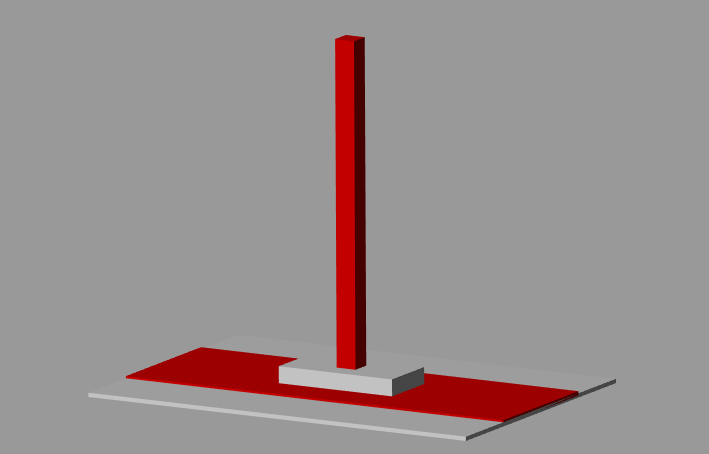
\includegraphics[width=0.95\linewidth]{../Analisis de Resultados/ImagenesAnalisis de Resultados/equilibrio.png}
  \caption{Simple.}
  \label{fig:sfig1}
\end{subfigure}%
\begin{subfigure}{.5\textwidth}
  \centering
  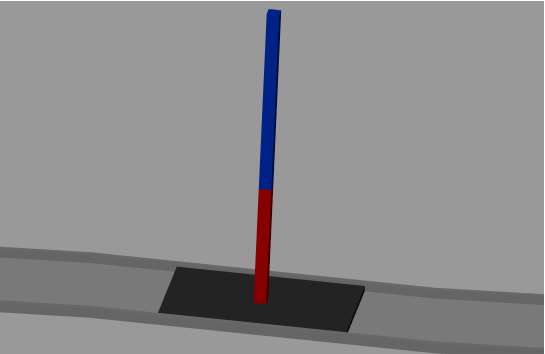
\includegraphics[width=0.95\linewidth]{../Analisis de Resultados/ImagenesAnalisis de Resultados/simscape_double_pendulum.png}
  \caption{Doble.}
  \label{fig:sfig2}
\end{subfigure}
\caption{Péndulo invertido.}
\label{fig:fig}
\end{figure}
Si bien esto es cierto, si se opta poro cambiar los parámetros de segundo, haciendo que el segundo link tenga una longitud que tienda a cero, ambos sistemas coinciden, como es de esperarse.

Si bien ambos sistemas son estrictamente observables en todos los casos de fricción tomando mediciones únicamente de la posición, por lo explicado anteriormente en la realidad realizar el control del péndulo doble midiendo únicamente la posición resulta mucho mas difícil, que en el caso del péndulo simple.
También resulta curioso que en el caso del péndulo simple, al ampliar el sistema para realizar el control integral el péndulo simple con roce y amortiguamiento resulta que no es controlable.
%\end{document}